We are now ready to perform the experiments. We will begin exploring SimCLR implementation and results, later we will explore BYOL's implementation and lastly we will compare them in order to see how BYOL tries to improve SimCLR and we will check if it successess or not.

The code used for the experimentations, as well as some files with the results, can be found on the Github repository for this work.

\section{SimCLR exploration}
We will perform an iterative exploration with this framework. We will explore a few range for a subset of the hyperparameters and then we will go deeper into some hyperparameters to try and obtain better results.

\subsection{First approach}
\label{experiments:simclr:first}

The first thing we did to experiment with this framework is to explore a wide range of hyperparameters to see which set of them performed better for us. The script that can be found in \lstinline{code/SimCLR/run.py}.

What we did for this first exploration was to define a \emph{parameter grid} and execute the whole framework using each combination of the parameters. The parameters that were firstly considerered are:
\begin{enumerate}
\item \lstinline{batch_size}. This is one of the most important parameters of SimCLR. In the original paper, it was proven that the higher this parameter, the better the results obtained for the linear classification. This parameter is also important since it has to adapt to our GPU's memory. The options that we have considered for the first experiments are: \lstinline|batch_size = {512,1024}|.

\item \lstinline{temperature}. The temperature parameter $\tau$ plays an important role in the individual loss seen in Equation \eqref{c:loss:simclr:ind}. It is suggested to try values in the range $[0,1]$ and the one that had better performance for the original experiments was around $0.5$, so we chose the following values: \lstinline|temperature = {0.25,0.5,0.75,1}|.

\item \lstinline{color_jitter_strength}. This parameter measures how hard is the color variation in the data augmentation. Previous results show that this parameter is important for the success of the network, so we provide with a big range of values. We include the following values: \lstinline|color_jitter_strength = {0.25,0.5,0.75,1}|.

\item \lstinline{epochs}. In the first stages of the experiments, we will always use $100$ as standard number of epoch for the trainings. We will see later if more epochs are needed in order to obtain better results.
\end{enumerate}

Using python and the python function \lstinline{itertools.product} we straightforwardly generate all possible different combinations of unions of the parameters so we only have to append them to a general string and execute the \lstinline{run.py} script mentioned before to obtain the results. In total, we obtain $32$ possible combinations, so we will obtain $32$ models. 

The script was executed and took approximately $24$ hours to train and evaluate all the different models, obtaining the results in Table \ref{table:simclr:gridsearch:1} in Appendix \ref{APPENDIX:B}. We have to remark, for each of the two possible batch sizes, the best results obtained. These are:

\begin{table}[H]
    \label{table:best:first:simclr}
\centering
\resizebox{\columnwidth}{!}{
\begin{tabular}{rrrrrrr}
batch\_size   & temperature   & color\_jitter & regularization\_loss & top\_1\_accuracy & top\_5\_accuracy & steps         \\ \hline
 512  &  0.25 &  0.25 &  0.0093      &  0.833         &  0.994          &  9800 \\
 1024 &    0.25       &  0.75 &  0.0093      &  \textbf{0.841}          &  0.995          &  4900 \\
\end{tabular}
}
\caption{Best results for the grid search experiment with SimCLR.}
\end{table}

\begin{remark}
On the original paper, the Top 1 accuracy score reported for CIFAR10 in $100$ epochs was $\sim 84.6\%$ accuracy for batch size $512$ and $\sim 85.1 \%$ accuracy score for $1024$ batch size. It has to be remarked that these results were obtained using ResNet-50,  larger version of ResNet. It is also reported that larger encoder architectures benefit the model, so this is an advantage they have at this point of the experiments . Having these aspects in account, and looking at the results obtained in our first experiment, we can say that this attempt was \emph{successfull}.
\end{remark}

Let us make some observations. The clearest is that, since the second batch size doubles the first one, the training ends in half the steps. We can see that the temperature obtained in both cases is the same, and it is equal to $0.25$. However, there is a big change in the color jitter parameter: while using $512$ as batch size obtains the best result with the value of $0.25$ for color jitter, using $1024$ as batch size this value changes to $0.75$, which implies stronger color changes on the data augmentation. 

In general, having a look again at the Table \ref{table:simclr:gridsearch:1} in Appendix \ref{APPENDIX:B},  we can see that:

\begin{itemize}
    \item As it also happens in the experiments made on the original SimCLR paper, lower temperature $\tau$ parameters cause higher accuracies on the linear heads of our models.
    
    \item The models perform better when the \lstinline{color_jitter} parameter is in the range $[0.5,0.75]$. This means that, in general, a generous amount of color jittering to our picture is benefitial for the models.

    \item The \emph{Top 5 accuracy} is above $99\%$ in each model. This says that, since the models almost always give the correct label one of the 5 highest values, but they obtain the correct tag around $84\%$ of the times, they might be creating some similar representations of the data for inputs that do not belong to the same class. 
\end{itemize}

\subsection*{Observations about the batch size}

Although both models get to the same value of regularization loss, the model with a batch size of $1024$ obtains a higher \emph{top 1 accuracy}. This seems to follow the intuitive idea that we presented before: SimCLR benefits from bigger batch sizes since it allows a positive sample to be compared and pushed appart from negative samples. Ideally, we would keep pushing the batch size parameter forward, doubling it again to try to find out if the performance of the model keeps benefiting from bigger batch sizes. However, this requires either using multiple GPUs(or TPUs) working in parallel on the training or using GPUs with bigger memory, which we do not have access to. 

Using the resources we have, the following experiment was performed: using the hyperparameters that we found out in our \emph{GridSearch} to be the ones that achieve the best results except for the \lstinline{batch-size}, we train models moving the batch size in the following range: 
$$
\text{\lstinline{batch-size}}=\{16,32,64,128,256,512,1024\},
$$
where the last two values had already been computed in the GridSearch so we do not have to repeat the training. 

\begin{remark}
    To avoid confusion, we have to remark that in the figures that will come in the next pages, all the models do not end the training in the same number of steps because the number of steps depends on the \lstinline{batch_size}. That does not mean that the models were trained for a different number of epochs, and the figures are presented like this because Tensorboard provides the charts using the steps in the $x$ axis. 
\end{remark}

\begin{figure}[htp] 
    \centering
    \subfloat[Evolution of the Top 1 accuracy with the batch size.]{%
        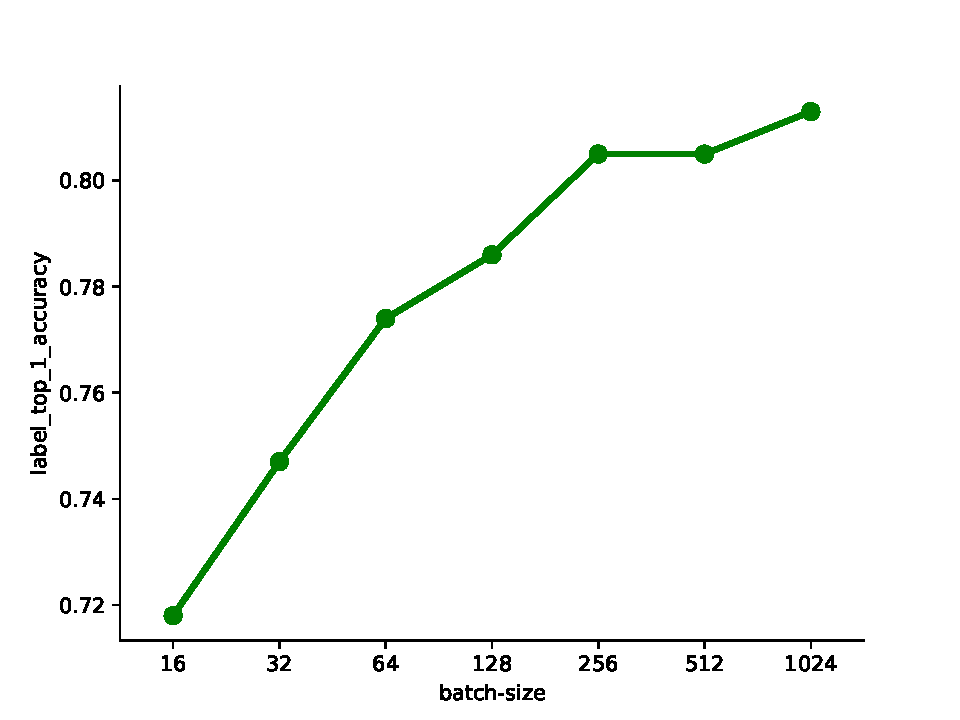
\includegraphics[width=0.45\textwidth]{simclr-batch-comparison}%
        \label{fig:accs:per:batch:simclr}%
        }%
    \hfill%
    \subfloat[Evolution curves of the accuracy with the steps taken in the training.]{%
        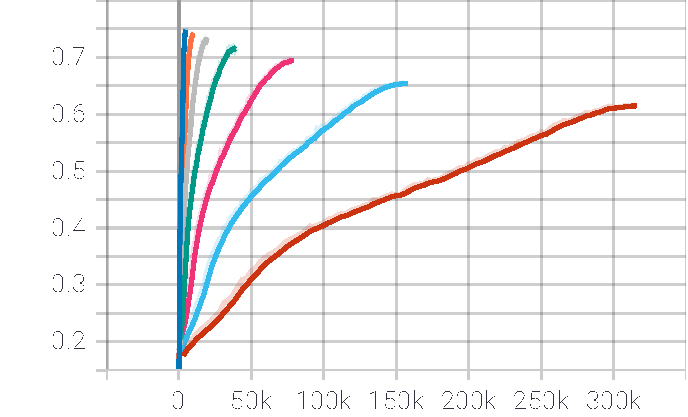
\includegraphics[width=0.45\textwidth]{train_supervised_acc}%
        \label{fig:evolution:acc:batches:simclr}%

        }%
        \caption{Results of the batch-size experiment.}
\end{figure}

Figure \ref{fig:accs:per:batch:simclr} shows the clear improvement of the Top 1 accuracy score when increasing the size of the batch that is used to compute the loss of our model. Increasing from $16$ to $1024$ gives an increase of more than $8\%$ in Top 1 accuracy, which is a lot. Further increase can be obtained if we keep increasing the batch size, but this is beyond our computation possibilities.

Figure \ref{fig:evolution:acc:batches:simclr} supports what we have just presented: not only with a smaller batch size we have to do thousands of extra steps in the training, but also we obtain much better accuracy performance of the linear head of the model.

\subsection*{Observations ofher hyperparameters}

We have seen that in our first experiment, batch size has been really relevant in the final results. We would like to see if the rest of the parameters play such an important role as well. 

As we have seen before, the parameters that we want to see how they affect the models are the \lstinline{color_jitter_strength} and the \lstinline{temperature} $\tau$ parameter. Let us study their impact on the model one by one. 

\begin{figure}[H] 
    \centering
    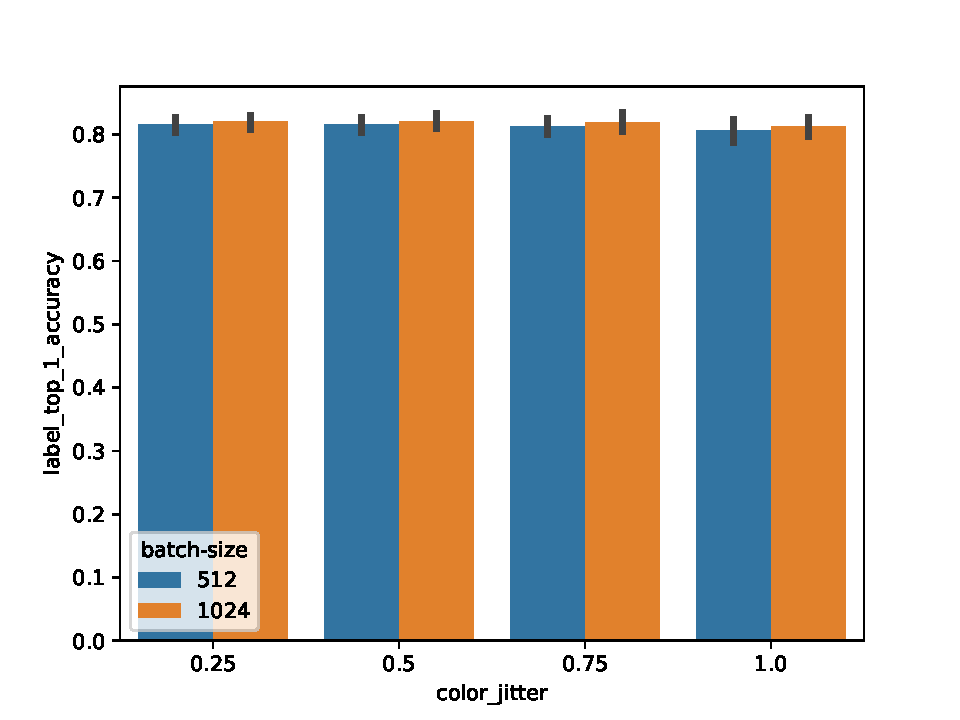
\includegraphics[width=0.55\textwidth]{color-jitter-impact-simclr}%
    
    \caption{Acurracy score following the color jitter parameter and both batch sizes considered.}
    
    \label{exp:simclr:colorjitter:impact}
\end{figure}

As we can see in Figure \ref{exp:simclr:colorjitter:impact}, the \lstinline{color_jitter_strength} parameter does not have a huge impact on the performance of the linear head of the model. The black bars on the center of each orange/blue bar indicate the variance of the accuracy respect the rest of the parameters. Surely, there are centesimal differences between the different values of this parameter. However, more finetuning might be needed in order to make this parameter relevant for our model. The low influence may as well be caused by the small encoder network (ResNet 18), so we will explore if there are any changes when we change the encoder network later in the document.

\begin{figure}[H] 
    \centering
        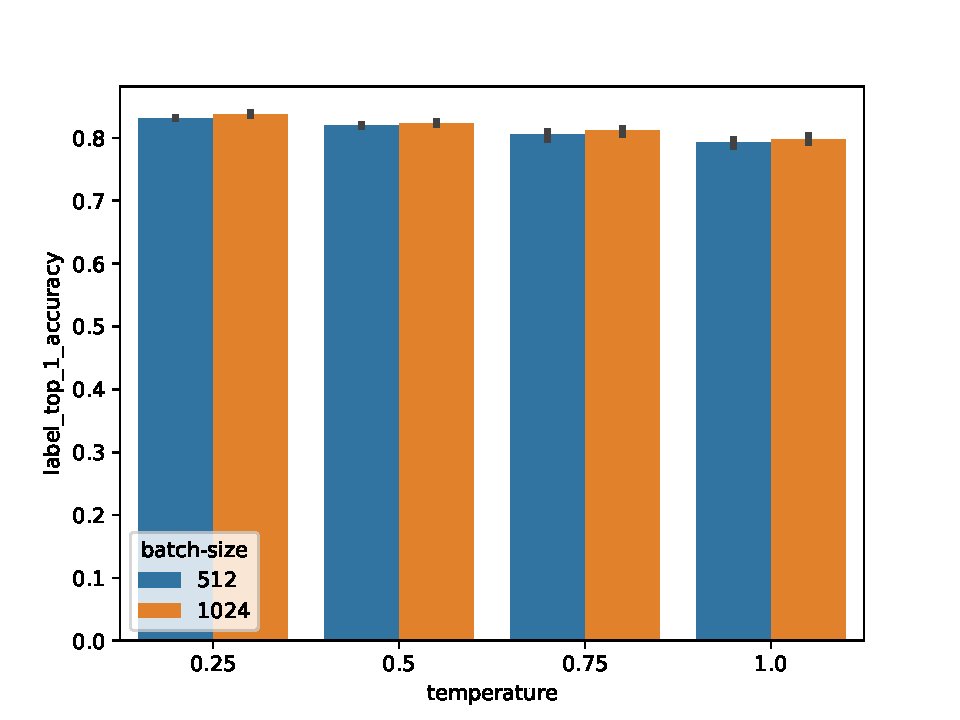
\includegraphics[width=0.55\textwidth]{temperature-impact-simclr}%
       
        \caption{Acurracy score following the temperature and both batch sizes considered.}
        
    \label{exp:simclr:temperature:impact}
\end{figure}

The parameter temperature, however, has a bigger impact on our framework's results. As we can see in Figure \ref{exp:simclr:temperature:impact}, when the temperature $\tau$ takes larger values, the accuracy obtained by the the linear head decreases. The decrease is approximately a $5\%$ on average, so we can affirm that the influence of the parameter is important on the model.

In the original paper, the best results also occurred with low values for the temperature parameter. They even tested lower values for this parameter and got even better results. We will have this in account for the following experiments.

\subsection{Going deeper on the encoder architecture}
\label{experiments:simclr:second}


As we have mentioned before, original results prove that using wider and deeper architectures for the encoder on the SimCLR framework. Going deeper, however, requires more computational capabilities since more parameters have to be adjusted.

In the implementation used, we have the option of changing an input parameter in order to execute the experiment with a different architecture for the encoder. Specifically, we can pass \lstinline{resnet_depth=50} as an argument to the \lstinline{run.py} script to execute the train of the framework and the linear head finetuning and evaluation with the Resnet50 architecture. The architecture for this neural network is presented in Table \ref{table:resnet:50}.


\begin{table}[H]
    \centering
    \begin{tabular}{|c|c|c|}
    \hline
    Layers                 & Output size                    & CIFAR10                         \\ \hline
    conv1                  & $112\times112$                 & $3\times3, \ 64,$ stride 1      \\ \hline
    \multirow{2}{*}{conv2} & \multirow{2}{*}{$56\times 56$} & $3\times3$ max pool, stride 2   \\ \cline{3-3} 
                           &                                & $\blockb{256}{64}{3}$           \\ \hline
    conv3                  & $28 \times 28$                 & $\blockb{512}{128}{4}$          \\ \hline
    conv4                  & $14 \times 14$                 & $\blockb{1024}{256}{6}$         \\ \hline
    conv5                  & $7 \times 7$                   & $\blockb{2048}{512}{3}$         \\ \hline
    \multirow{2}{*}{}      & $1\times 1$                    & $7\times 7$ global average pool \\ \cline{2-3} 
                           &                                & $10-d$ FC, softmax              \\ \hline
    \multicolumn{2}{|c|}{Number of parameters}              & $23.520.842$                    \\ \hline
    \end{tabular}
    \caption{Resnet50 architecture.}
    \label{table:resnet:50}
\end{table}

    As we can see comparing this architecture with ResNet18 in Table \ref{arch:resnet:18}, the number of parameters that the network has to train doubles the first one, so we expect to have less memory available on our GPU so the \lstinline{batch_size} will have to be decreased to be able to run the trainings. 
    
    This is clearly an issue, since we have already shown empirically that our model benefits from taking larger values on this parameter. In this second stage of exploring the best parameters for SimCLR on CIFAR10, we used the following parameters set to perform our particular GridSearch:
    
    \begin{itemize}
        \item \lstinline{batch_size}. In this second experiment, due to the limitations in the GPU memory, we have to reduce the range of this parameter to:
        $$
        \text{\lstinline{batch-size}}=\{16,32,64,128,256\}.
        $$

        \item \lstinline{temperature}. We found out that, as it happens also to the original paper's experiments, lower temperature values help our representations to be better for downstream tasks. However, we decided to try again \emph{higher} temperature values again, that is: temperature values in the set $\{0.5,0.75\}$, to explore if the temperature parameter had any correlation with the encoder architecture.
        
        \item \lstinline{color_jitter_stregth}. This time we focus on harder (higher) color jitter strengths, testing in the range $\{0.65,0.75\}$, since in the first experiments the results obtained were better when this parameter was higher.
        
\end{itemize}

    Using this parameters, our script to train and evaluate the models using each combination was executed. The results obtained can be checked in Table \ref{table:simclr:gridsearch:2} in Appendix \ref{APPENDIX:B}. We remark in Table \ref{table:best:second:simclr} some of the most interesting results, comparing them with the ones obtained in the first experiment.

    \begin{table}[H]
        \label{table:best:second:simclr}
    \centering
    \resizebox{\columnwidth}{!}{
    \begin{tabular}{lrrrrrrr}
    Experiment & batch\_size   & temperature   & color\_jitter & regularization\_loss & top\_1\_accuracy & top\_5\_accuracy & steps         \\ \hline
    1st & 512  &  0.25 &  0.25 &  0.0093      &  0.833         &  0.994          &  9800 \\
    1st & 1024 &    0.25       &  0.75 &  0.0093      &  0.841          &  0.995          &  4900 \\
    2nd & 128 & 0.5 & 0.65 & 0.0225 & 0.844 & 0.994 & 39100 \\
    \textbf{2nd} & \textbf{256} & \textbf{0.5} & \textbf{0.75} & \textbf{0.023} & \textbf{0.848} & \textbf{994} & \textbf{19695} 
    \end{tabular}
    }
    \caption{Best results for the second grid search experiment with SimCLR.}
    \end{table}

    As we can see, the results of the models that use ResNet50  as an encoder outperform for a few hundredths in the Top 1 Accuracy score, and also they reach a lower loss function. Since it is clear that the gain we obtain by increasing the encoder depth is minimal, we may think that it is not worth it for our model since the number of parameters that have to be trained and, thus, the time that the train takes is much higher. However, we must not forget a very important fact that we observed in the first experiment: SimCLR benefits from bigger batch sizes. The results are comparing batch sizes $512$ and $1024$ in the first experiment with $128$ and $256$ in the second experiment (as we have already mentioned, the GPU memory does not allow us to use a bigger batch size when we increase the encoder depth).

    Taking this into account and although we can not empirically prove it, we state that when the batch size is increased as well as the encoder depth, the models with larger depth will outperform the models using ResNet18. Let us see some more details about the training.

    In the official implementation of SimCLR, two losses are computed: a contrastive loss and a supervised loss. The total loss is computed as the sum of both:
    \[
    \mathcal L_{tot} = \mathcal L_{contrastive} + \mathcal L_{supervised}.    
    \]

    We can visualize how the loss evolve through the training using the Tensorboard output. The lines are smoothed, that is why sometimes there might be some \emph{shadows} near the lines. The coefficient of smoothing is set as default ot $0.6$. 
    \begin{figure}[htp] 
        \centering
        \subfloat[Contrastive loss in train]{%
            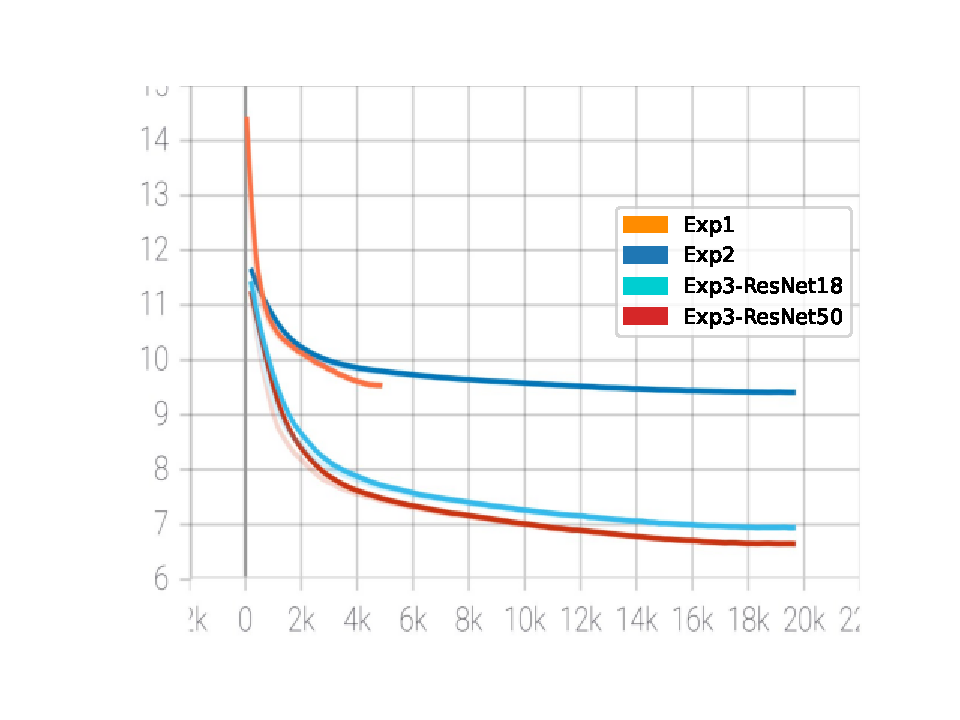
\includegraphics[width=0.45\textwidth]{simclr-exp2/train_contrast_loss}%
            \label{fig:contrastive:loss:exp2}%
            }%
        \hfill%
        \subfloat[Supervised loss in train]{%
            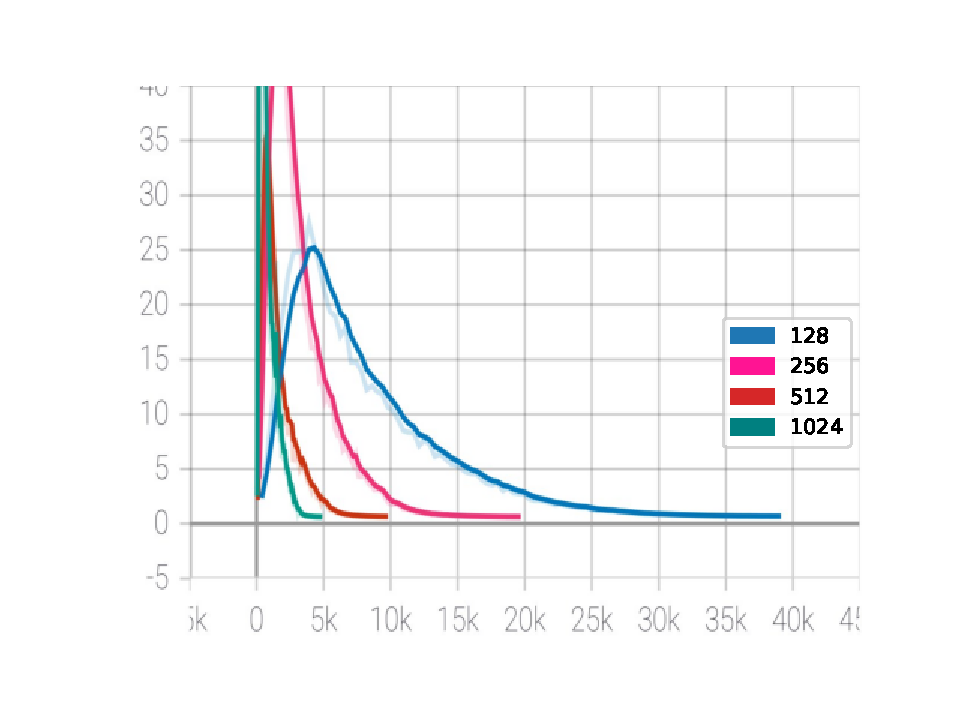
\includegraphics[width=0.45\textwidth]{simclr-exp2/train_supervised_loss}%
            \label{fig:supervised:loss:exp2}%
    
            }%
            \caption{Graphs on the losses during trian in second experiment. On axis $x$ we have the number of steps and on $y$ axis the value of the loss.}
            \label{fig:exp2:both:losses}
    \end{figure}


\begin{figure}[H]
\centering
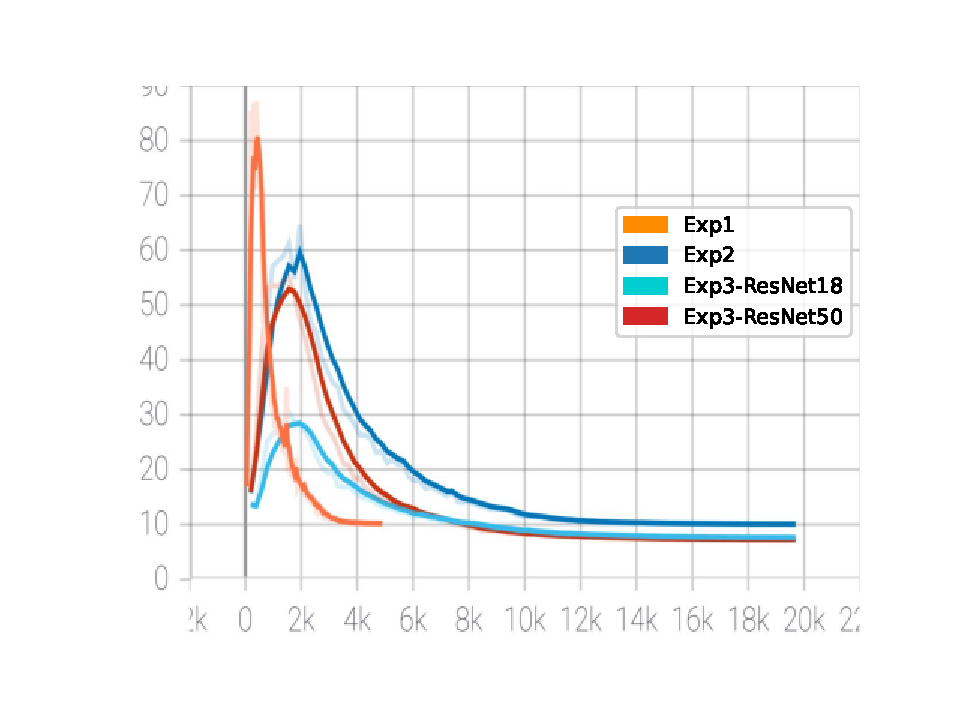
\includegraphics[width=0.55\textwidth]{simclr-exp2/train_total_loss}%
\caption{Total loss of the four remarked models in the second experiment. The axis are the same of the ones in Figure \ref{fig:exp2:both:losses} }
\label{fig:total:loss:exp2}%
\end{figure}

As we can see, although the loss is a sum of two components, as the steps/epochs get close to the end of the training, the supervised loss tends to zero. However, the contrastive loss remains in the range $[8,9.5]$ approximately. 

If we have a look at Figure \ref{fig:supervised:loss:exp2} we can see that in all cases it reaches a minimum and although more steps of the experiments are done, the value of this loss does not get reduced. Hoewever, if we have a look at the contrastive loss in Figure \ref{fig:contrastive:loss:exp2}, we can see that in three out of the four models, the loss is still decreasing and if we increased the number of epochs,we state that we would probably obtain better results.

\subsection{Gaussian blur in the image augmentations}

We have also studied if adding \emph{gaussian blur} as a part of the data augmentation process. This can be easily done by adding the parameter \lstinline{--use_blur=True} to the run script.